%----------------------------------------------------------------------------------------
%	Metropolia Thesis LaTeX Template
%----------------------------------------------------------------------------------------
% License:
% This work is licensed under the Creative Commons Attribution 4.0 International License. To view a copy of this license, visit http://creativecommons.org/licenses/by/4.0/.
%
% Authors:
% Panu Leppäniemi, Patrik Luoto and Patrick Ausderau
%
% Credits:
% Panu Leppäniemi: abstract, def, cleaning,...
% Patrik Luoto: title page, abstract in Finnish, abbreviation, math,...
% Patrick Ausderau: initial version, style, table of content, bibliography, figure, appendix, table, source code listing...
%
% Please:
% If you find mistakes, improve this template and alike, please contribute by sharing your improvements and/or send us your feedback there: https://github.com/panunu/metropolia-thesis-latex
% And of course, if you improve it, add yourself as an author.
%
% Compiler:
% Use XeLaTeX as a compiler.

%----------------------------------------------------------------------------------------
%    ToDo
%----------------------------------------------------------------------------------------
% % % TÄRKEÄT
% % Odotetaan 29.11.2013 asti äikänmaikkojen ja viestinnän mahdollisia kommentteja.
%   %done?
%
% % % Vähemmän tärkeät

 
%----------------------------------------------------------------------------------------
%	TITLE PAGE CONFIGURATION
%----------------------------------------------------------------------------------------

\def\thesislang{english} %change this depending on your language
\author{Álvaro Bolaños Rodríguez}
\def\thesis{Opinnäytetyö/Thesis}
\def\alaotsikko{Creating a cloud based communication channel}

%Finnish section
\def\otsikko{Opinnäytetyön otsikko}
\def\tutkinto{Tutkinto}
\def\kohjelma{Koulutusohjelma}
\def\suuntautumis{Suuntautumisvaihtoehto}
\def\ohjaajat{
Etunimi Sukunimi, Titteli\newline
Etunimi Sukunimi, Titteli
}
\def\avainsanat{avainsanat}
\def\pvm{\specialdate\today}

%English section, for abstract
\title{IR camera in Well-being technology}
\def\metropoliadegree {Bachelor of Engineering}
\def\metropoliadegreeprogramme {Information Technology}
\def\metropoliaspecialisation {Software Engineer}
\def\metropoliainstructors {
Name, Title \newline
}
\def\metropoliakeywords {Keywords}
\date{\today}

%----------------------------------------------------------------------------------------
%	GLOBAL STYLES
%----------------------------------------------------------------------------------------

\documentclass[hidelinks,11pt,a4paper,oneside,article]{memoir}
\usepackage[\thesislang]{babel} 
\usepackage{iflang}
\usepackage{amsmath}
\usepackage{amsfonts}
\usepackage{amssymb}
\usepackage{fontspec}
\usepackage{tocloft}
\usepackage{titlesec}
\usepackage[hyphens]{url}
\usepackage{mathtools}
\usepackage{wallpaper}
\usepackage{datetime}
\usepackage[bookmarksdepth=subsection]{hyperref} % for automagic pdf links for toc, refs, etc.
\usepackage[amssymb]{SIunits}
\usepackage[version=3]{mhchem}
\usepackage{pgfplots} %simple plots etc
\usepackage{pgfplotstable}
\usepackage{tikz} % mindmaps, flowcharts, piecharts, examples at http://www.texample.net/tikz/examples/
\usepackage{csquotes}
\usetikzlibrary{shapes.geometric, arrows}
\numberwithin{equation}{chapter}


\renewcommand{\dateseparator}{.}
%condition for adding or not space in TOC
\usepackage{etoolbox}
%for compact list
\usepackage{enumitem}
%for block comment
\usepackage{verbatim}
%for "easier" references
\usepackage{varioref}
%forcing single line spacing in bibliography
\DisemulatePackage{setspace}
\usepackage{setspace}
%including figure (image)
\usepackage{graphicx}
%change the numbering for figure
\usepackage{chngcntr}
%strike trough
\usepackage{ulem}
%euro symbol
\usepackage{eurosym}
%try to count
\usepackage{totcount}
%insert source code
\usepackage{listings}
\usepackage[justification=justified,singlelinecheck=false]{caption}
\usepackage{color}
%force the width of a table instead of column
\usepackage{tabularx}
\usepackage{booktabs} %why not booktabs? :3
% Abbreviations, acronym and glossary
\usepackage[acronym,nonumberlist,section]{glossaries}%xindy,%toc, ,nomain

\usepackage{float} % For forced figure location with modifier H (\begin{figure}[H])
\usepackage{cite} % Make citations to match Metropolia thesis guide

% change font of links in bibliography to same as other text
\usepackage{url}
\urlstyle{same}

% change punctuation of multiple cites to semicolon instead of comma: [1; 2; 3]
\renewcommand\citepunct{; }

% citep-macro for reference with period inside square brackets [1.]
\newcommand{\citep}[1]{
 \renewcommand\citeright{.]}
 \cite{#1}
 \renewcommand\citeright{]}
}

%set date format to D.M.YYYY
\newdateformat{specialdate}{\THEDAY.\THEMONTH.\THEYEAR}

\newcommand\tn[1]{\textnormal{#1}} %use \tn instead of \textnormal
\newcommand\reaction[1]{\begin{equation}\ce{#1}\end{equation}} %\reaction{} for chemical reactions

%NORMAL TEXT
%all text, title, etc. in the same font: Arial
%replace with arial.ttf if you have the fontfile
\setmainfont
[BoldFont=LiberationSans-Bold.ttf,
ItalicFont=LiberationSans-Italic.ttf,
BoldItalicFont=LiberationSans-BoldItalic.ttf]
{LiberationSans-Regular.ttf}
%line space
\linespread{1.5}
%\doublespacing
%margin
\usepackage[top=2.5cm, bottom=3cm, left=4cm, right=2cm, nofoot]{geometry}
\setlength{\parindent}{0pt} %first line of paragraph not indented
\setlength{\parskip}{16.5pt} %one empty line to separate paragraph
%list with small line space separation
\tightlists

%IMAGE - FIGURE
%the figures should be placed in the "illustration" folder
\graphicspath{{illustration/}}
%figure number without chapter (1.1, 1.2, 2.1) to (1, 2, 3)
\counterwithout{figure}{chapter}
%border around images
\setlength\fboxsep{0pt}
\setlength\fboxrule{0.5pt}
%caption font size
\captionnamefont{\small}
\captiontitlefont{\small}
%space after figure caption (and other float elements)
\setlength{\belowcaptionskip}{-7pt}

%TABLE
\counterwithout{table}{chapter}

%SOURCE CODE
\definecolor{darkgray}{rgb}{.4,.4,.4}
\definecolor{purple}{rgb}{0.65, 0.12, 0.82}
\lstset{
extendedchars=true,
captionpos=b,
caption=\footnotesize,
basicstyle=\singlespacing\ttfamily,%\small\fontfamily{"Courier"}\selectfont,
keywordstyle=\color{blue}\bfseries,
commentstyle=\color{purple}\itshape,
identifierstyle=\color{black},
stringstyle=\color{red},
showstringspaces=false,
showspaces=false,
numbers=left,
numberstyle=\footnotesize,
numbersep=9pt,
breaklines=true,
tabsize=2,
showtabs=false,
xleftmargin=1cm
}
\IfLanguageName {finnish} {\renewcommand{\lstlistingname}{Listaus}} {} % what is a good translation for this?
%\counterwithout{lstlisting}{chapter}
%moved after begin document, otherwise does not compile

%% set this format as the default for lstlisting
%\DeclareCaptionFormat{empty}{}
%\captionsetup[lstlisting]{format=empty}

%TOC
%change toc title
\IfLanguageName {finnish} {\addto{\captionsfinnish}{\renewcommand*{\contentsname}{Sisällys}}} {}
%remove dots
\renewcommand*{\cftdotsep}{\cftnodots}
%chapter title and page number not in bold
\renewcommand{\cftchapterfont}{}
\renewcommand{\cftchapterpagefont}{}
%sub section in toc
\setcounter{tocdepth}{2}
%subsection numbered
\setcounter{secnumdepth}{2}
\renewcommand{\tocheadstart}{\vspace*{-15pt}}
\renewcommand{\printtoctitle}[1]{\fontsize{13pt}{13pt}\bfseries #1}
\renewcommand{\aftertoctitle}{\vspace*{-22pt}\afterchaptertitle}
%spacing afer a chapter in toc
\preto\section{%
  \ifnum\value{section}=0\addtocontents{toc}{\vskip11pt}\fi
}
%spacing afer a section in toc
\renewcommand{\cftsectionaftersnumb}{\vspace*{-3pt}}
%spacing afer a subsection in toc
\renewcommand{\cftsubsectionaftersnumb}{\vspace*{-1pt}}
%appendix in toc with "Appendix " + num
\IfLanguageName {finnish} {
  \renewcommand*{\cftappendixname}{Liite\space}
  \renewcommand{\appendixtocname}{Liitteet}
}{\renewcommand*{\cftappendixname}{Appendix\space}}
%appendix header
\IfLanguageName {finnish} {\def\appname{Liite\space}}{\def\appname{Appendix\space}}

%TITLES
%chapter title
\titleformat{\chapter}
{\fontsize{13pt}{13pt}\bfseries\linespread{1}}
{\thechapter}{.5cm}{}
\titlespacing*{\chapter}{0pt}{.32cm}{9pt}
\titleformat{\section}
{\fontsize{12pt}{12pt}\linespread{1}}
{\thesection}{.5cm}{}
\titlespacing*{\section}{0pt}{14pt}{6pt}
\titleformat{\subsection}
{\fontsize{12pt}{12pt}\linespread{1}}
{\thesubsection}{.5cm}{}
\titlespacing*{\subsection}{0pt}{14pt}{6pt}


%QUOTE
\renewenvironment{quote}
  {\list{}{\rightmargin=0pt\leftmargin=1cm\topsep=-10pt}%
  \item\relax\fontsize{10pt}{10pt}\singlespacing}
  {\endlist}

%BIBLIOGRAPHY
%bibliography title to be "references"
%if the title don't get renamed properly, move that line after the \begin{document}
\IfLanguageName {finnish} {\addto{\captionsfinnish}{\renewcommand*{\bibname}{Lähteet}}} {\renewcommand\bibname{References}}
\makeatletter %reference list option change
\renewcommand\@biblabel[1]{#1\hspace{1cm}} %from [1] to 1 with 1cm gap
\makeatother %
\setlength{\bibitemsep}{11pt}

%count the appendices (since the chapter counter is reset after \appendix).
%! require to complie 2 times
\regtotcounter{chapter}

%ABBREVIATION AND GLOSSARY
% Generate the glossary
\makeglossaries

%Acronyms, abbreviations, etc. definitions
\newacronym{html}{HTML}{HyperText Markup Language}
\newacronym{sql}{SQL}{Structured Query Language}
\newacronym{io}{I/O}{Input/Output}
\newacronym{ram}{RAM}{Random Access Memory}
\newacronym{php}{PHP}{Hypertext Preprocessor}
\newacronym{lte}{LTE}{Long Term Evolution}
\newacronym{3g}{3G}{Third generation}
\newacronym{ir}{IR}{Infrared}
\newacronym{iot}{IoT}{Internet of Things}
\newacronym{usb}{USB}{Universal Serial Bus}
\newacronym{sim}{SIM}{subscriber identity module}
\newacronym{spi}{SPI}{Serial Peripheral Interface}
\newacronym{api}{API}{Application Program Interface}
\newacronym{otg}{OTG}{USB On-The-Go}
\newacronym{ui}{UI}{User Interface}
\newacronym{http}{http}{Hypertext Transfer Protocol}
\newacronym{java}{Java}{Java language}
\newacronym{javame}{Java ME}{Java Micro Edition}



%Glossary entries
\newglossaryentry{part_key}{
	name={partition key}, 
	description={a column or set of columns from the same table whose consolidated value decide the partition for a given data}
}
\newglossaryentry{thesis}{
	name=thesis, 
	description={a written essay one submitted for a university degree},
	plural=theses
}
\newglossaryentry{latex}
{
    name=\LaTeX{},
    description={Is a mark up language specially suited for scientific documents}
}
 
\newglossaryentry{maths}
{
    name=mathematics,
    description={Mathematics is what mathematicians do}
}

%----------------------------------------------------------------------------------------
%	TITLE PAGE
%----------------------------------------------------------------------------------------
\makeatletter
\renewcommand{\maketitle}{
\thispagestyle{empty}
\ThisCenterWallPaper{1}{viiva}
%
\vspace*{9.5cm}
\tn{\LARGE\@author\\[22pt]\Huge\IfLanguageName {finnish}{\otsikko}{\@title}\\[22pt]\LARGE\alaotsikko\\[1.75cm]}

\parbox{.7\linewidth}{
\IfLanguageName {finnish}{
  Metropolia Ammattikorkeakoulu\\
  \tutkinto \\
  \kohjelma \\
  \thesis\\
  \pvm
} {
  Helsinki Metropolia University of Applied Sciences\\
  \metropoliadegree \\
  \metropoliadegreeprogramme \\
  \thesis\\
  \specialdate\today % D.M.YYYY date format
}
}
\ThisLRCornerWallPaper{1}{metropolia}
%
\clearpage
}
\makeatother

\makepagestyle{tiivis}
\makeevenhead{tiivis}{}{}{Tiivistelmä}
\makeoddhead{tiivis}{}{}{Tiivistelmä}

\makepagestyle{abstract}
\makeevenhead{abstract}{}{}{Abstract}
\makeoddhead{abstract}{}{}{Abstract}

\begin{document}
\counterwithout{lstlisting}{chapter}

%page number always on the top right, clear the "chapter/section" head
\pagestyle{myheadings}
\markright{}
%clear chapter "title" foot page
\makeevenfoot{plain}{}{}{}
\makeoddfoot{plain}{}{}{}



\maketitle
\newpage
\LRCornerWallPaper{1}{footer}

%----------------------------------------------------------------------------------------
%	ABSTRACT
%----------------------------------------------------------------------------------------

\pagestyle{abstract}
\begin{tabular}{ | p{4,7cm} | p{10,3cm} |}
  \hline
  Author(s) \newline
  Title \newline\newline 
  Number of Pages \newline
  Date
  & 
  \makeatletter
  \@author \newline
  \@title \newline\newline
  \pageref*{LastPage} pages + \total{chapter} appendices \newline %! if no appendices, risk to count total of chapter :D
  \IfLanguageName {finnish} {\foreignlanguage{english}{\longdate\@date}} {\@date}
  \makeatother
  \\ \hline
  Degree & \metropoliadegree
  \\ \hline
  Degree Programme & \metropoliadegreeprogramme
  \\ \hline
  Specialisation option & \metropoliaspecialisation
  \\ \hline
  Instructor(s) & \metropoliainstructors
  \\ \hline
  \multicolumn{2}{|p{15cm}|}{\begin{singlespacing}\vspace{-22pt}
  \paragraph{}	
  In this bachelor's thesis project I develop a communication system for \gls{ir} cameras using \gls{iot} modules to connect them to mobile networks through \gls{lte} hence to Internet, a server-side will receive, analyses and configures ir cameras and send to data to clients
  \paragraph{}
  One of the key points using \gls{ir} cameras is the respect of privacy, Unlike normal cameras generally people cannot be recognized. Applications are related to monitoring of patients: trigger alarm when a patient does not move for a while, control the number of people in a room, etc.
  \paragraph{}
  This project is focused on the technical details of the communication system and implements what was studied on my Innovation Project, specifically analysis techniques that can be done on the server-side.
  
  \end{singlespacing}} \\[14cm] \hline
  Keywords & \metropoliakeywords
  \\ \hline
\end{tabular}
\clearpage

%----------------------------------------------------------------------------------------
%	Acknowledgement ?
%----------------------------------------------------------------------------------------
%\chapter*{Acknowledgement}
%Thanks to my cat
%\clearpage

%----------------------------------------------------------------------------------------
%	TABLE OF CONTENTS
%----------------------------------------------------------------------------------------

\makeevenhead{plain}{}{}{}
\makeoddhead{plain}{}{}{}
\pagestyle{empty} %remove page number in toc (if longer than 2 pages)
\tableofcontents*
\pagestyle{empty} %remove page number in toc (if longer than 1 pages)


\clearpage
%Uncomment this line if you do not have Abbreviations list.
%\pagestyle{plain}

%list of figure, tables comes here...


%----------------------------------------------------------------------------------------
%    Lyhenteet / Abbreviation
%----------------------------------------------------------------------------------------

\begin{singlespacing}

\glsaddall

{
	\titleformat{\section}
	{\fontsize{13pt}{13pt}\bfseries\linespread{1}}
	{\thesection}{.5cm}{}
	%Adapt labelwidth (sorry for the ugly hack)
	\setlist[description]{leftmargin=!, labelwidth=4em}
	\IfLanguageName {finnish} {
		\printacronyms[title=Lyhenteet]
	}{
		\printacronyms[title=Abbreviations]
	}
	\setlist[description]{leftmargin=!, labelwidth=7em}
	\printglossary 
	\setlist[description]{style=standard} % reset settings back to default
}
\end{singlespacing}
%Seems that bug is in sharelatex. Compile fine with TexLive >= 2014


\newpage

%page number always on top right; also for chapter "title" page
\pagestyle{plain}
\makeevenhead{plain}{}{}{\thepage}
\makeoddhead{plain}{}{}{\thepage}

\setcounter{page}{1} %page 1 should be Introduction
\ClearWallPaper
%----------------------------------------------------------------------------------------
%	CONTENT
%----------------------------------------------------------------------------------------

\sloppy % enforce alignment to fully justified

\chapter{Introduction}


Thermal images had a number of advantages over conventional light-based video camera images. These thermal images tell us not only there are living people or animals but also if there is any temperature anomaly on them. They can be used to make assumptions about their physical state using image processing software.

Here is where \gls{iot} comes into play, Nowadays the Internet is very accessible and fast. Almost every conceivable device: phones, watches, televisions, speakers, cameras, etc can be connected, send and receive continuously big amounts of data.

Although with \gls{iot} it comes the inevitable process of define a communication channel between the \gls{iot} devices, visualize, store and distribute data from them. On this paper it is explained the steps of how to develop software solutions to these topics and all the alternatives that were tried, which ones and why were implemented at the end along all the tools and technologies which were used to carry out the project as smoothly as possible.


%% imporve this
Finland is nowadays facing a difficult issue in the area of well-being. The population is aging and the costs in elder health and mental health care are sky-rocketing. This is why health care entities in Finland are looking into decrease their costs by search for new ideas in the field of IT.
This thesis discusses also how \gls{ir} sensors could be exploited in the case company to decrease costs and improving monitoring of patients.

\section{Background of the case company}
The thesis originates in a project I am doing in collaboration with a startup called Levitezer (\url{http://www.levitezer.com/}). A company that develops gimbals and controllers for cameras for image stabilization among other projects \cite{levitezer}.

Even though this is not a health care company, the sensors and methods here explained could be used in Hospitals, sanatoriums, clinics, nursing homes, etc. And right now Levitezer is trying to expand their business to other areas.

The methods and software I developed are being used to create an \gls{api} that connect \gls{ir} sensors together.

\section{Business Challenge}
%% improving costs by not having personal watching people all the time
Find a system which using \gls{ir} sensors allow us to monitoring patients while keeping their privacy along reducing costs by using less staff and improve the service quality, data from those sensors can be accessed from anywhere which make them very versatile and portable.
\section{Objective and Outcome of the Study}
With the business challenge in mind, this study aims to answer the following question:
\begin{displayquote}
{\large  How to create a effective communication channel between ir sensors and clients such as computers, laptops, etc and use it on Well-being services?}
\end{displayquote}

The outcome of this study is a full working communication Chanel using modern cloud technologies, client-side pieces of software able to read sensors; displaying data in form of images while receiving commands to change the sensor behavior, all in bidirectional full duplex communication, proposals to use it on health care institutions and use cases for image analysis
This is an great project as it is a hot topic (\gls{iot} and cloud computing) in the IT world. Methods described on this thesis may help others with their projects.


\chapter{Theoretical Background}
%What is already known about your chosen subject area and what is not known?
%Discuss ideas in previous studies relevant to your topic (a brief introduction to the current state of knowledge and practice in your subject area). Identify a gap in the subject area and justify the purpose of your project, that is, the focus of your topic.


%Streaming serial data (binary) from IR camera using android devices and \gls{lte} modules to cloud,
%and from cloud to clients that wish to listen the stream (to see ir camera).



\subsection{Raspberry Pi and Lte dongle}

\section{Connectivity Methods: protocols}

\subsection{UDP}

\subsubsection{The NAT problem}

\subsection{http/s}
\cite{http-rfc}

\subsection{Websockets}
\cite[p.~30]{rfc6455}




\chapter{Methods and Materials}
%How was the project carried out in practice, and how was the data analysed?
%Describe the context in which the work was carried out (such as the overall project and its design, your specific task, work environment) and the workflow. Describe the methods and materials used (accurate details of data, software, materials, methods, techniques). Give a full account of exact test arrangements and measurements carried out, and accurate details of data analysis.
%The issues included in this section depend on the nature of your project. Whatever the issues, describe them in sufficient detail and in logical sequence.


\section{The sensor}
This project started with a \gls{ir} sensor provided by Levitezer which delivers all infrared data in form of binary streams trough \gls{usb}.

 In order to make the an image with some sort of programing language it is necessary to process the those streams. Every image or frame comes in 240 chunks or rows separated by a sequence of 3 bytes:

\begin{equation}
\label{eq:stream of data}
\text {FF FF FF 00} \left\lbrace data \right\rbrace 
\text {FF FF FF 01} \left\lbrace data \right\rbrace 
\text {FF FF FF 02} \left\lbrace data \right\rbrace \dots
\end{equation}



In 3.1 every byte is seen in hexadecimal format containing an sequence "FF FF FF" is the between rows of typically 80 bytes of data. After the sequence, the 4th byte is the number which identify the row.

The 240th (F0 in hexadecimal) row provides meta-data about the frame

\begin{equation}
\label{eq:metadata row}
\dots \text {FF FF FF F0} \left\lbrace data \right\rbrace
\end{equation}

% Description of the telemetry



\section{Reading the sensor Methods}
A number of reading methods were tried, some worked better than others

\subsection{Android smart-phone as Gateway}
Most of Android smartphones have an \gls{otg} which allows to use usb peripherals in the phone with the correspondent \gls{otg} adaptator. This can be used to develop an Android application to receive the data from the sensor and send it through Internet using any protocol.


This was tested using a \gls{php} file in a server on Metropolia UAS alongside an Android Application I developed to send all the data from the sensor to server, this application is available in GitHub on the following link. %link!!!
 
In order to send data to the cloud a path must be done. The first approach was connect the sensor to an Android smart-phone to use it as a gateway to Internet, letting the sensor access the \gls{3g} or the \gls{lte} network

This method requires to code an Android Application using Java and the Android framework, also requires a terminal which supports \gls{otg} \gls{usb}. For this purpose a library to read binary data from the \gls{usb} will be of great help. This is one open-source that can be accessed: \url{https://github.com/mik3y/usb-serial-for-android}

A good thing about this approach is that we already have all the hardware to do the communication so that there is only need to focus on the software part.

\subsubsection{Description of the Android Application}
To create the Android application it is needed some things:
\begin{itemize}
	\item A minimal \gls{ui}
	\item A network protocol and its implementation
	\item A background process
\end{itemize}

The \gls{ui} let us start the reading and provide an address and a port to connect.


\begin{figure}[h]
	\centering
	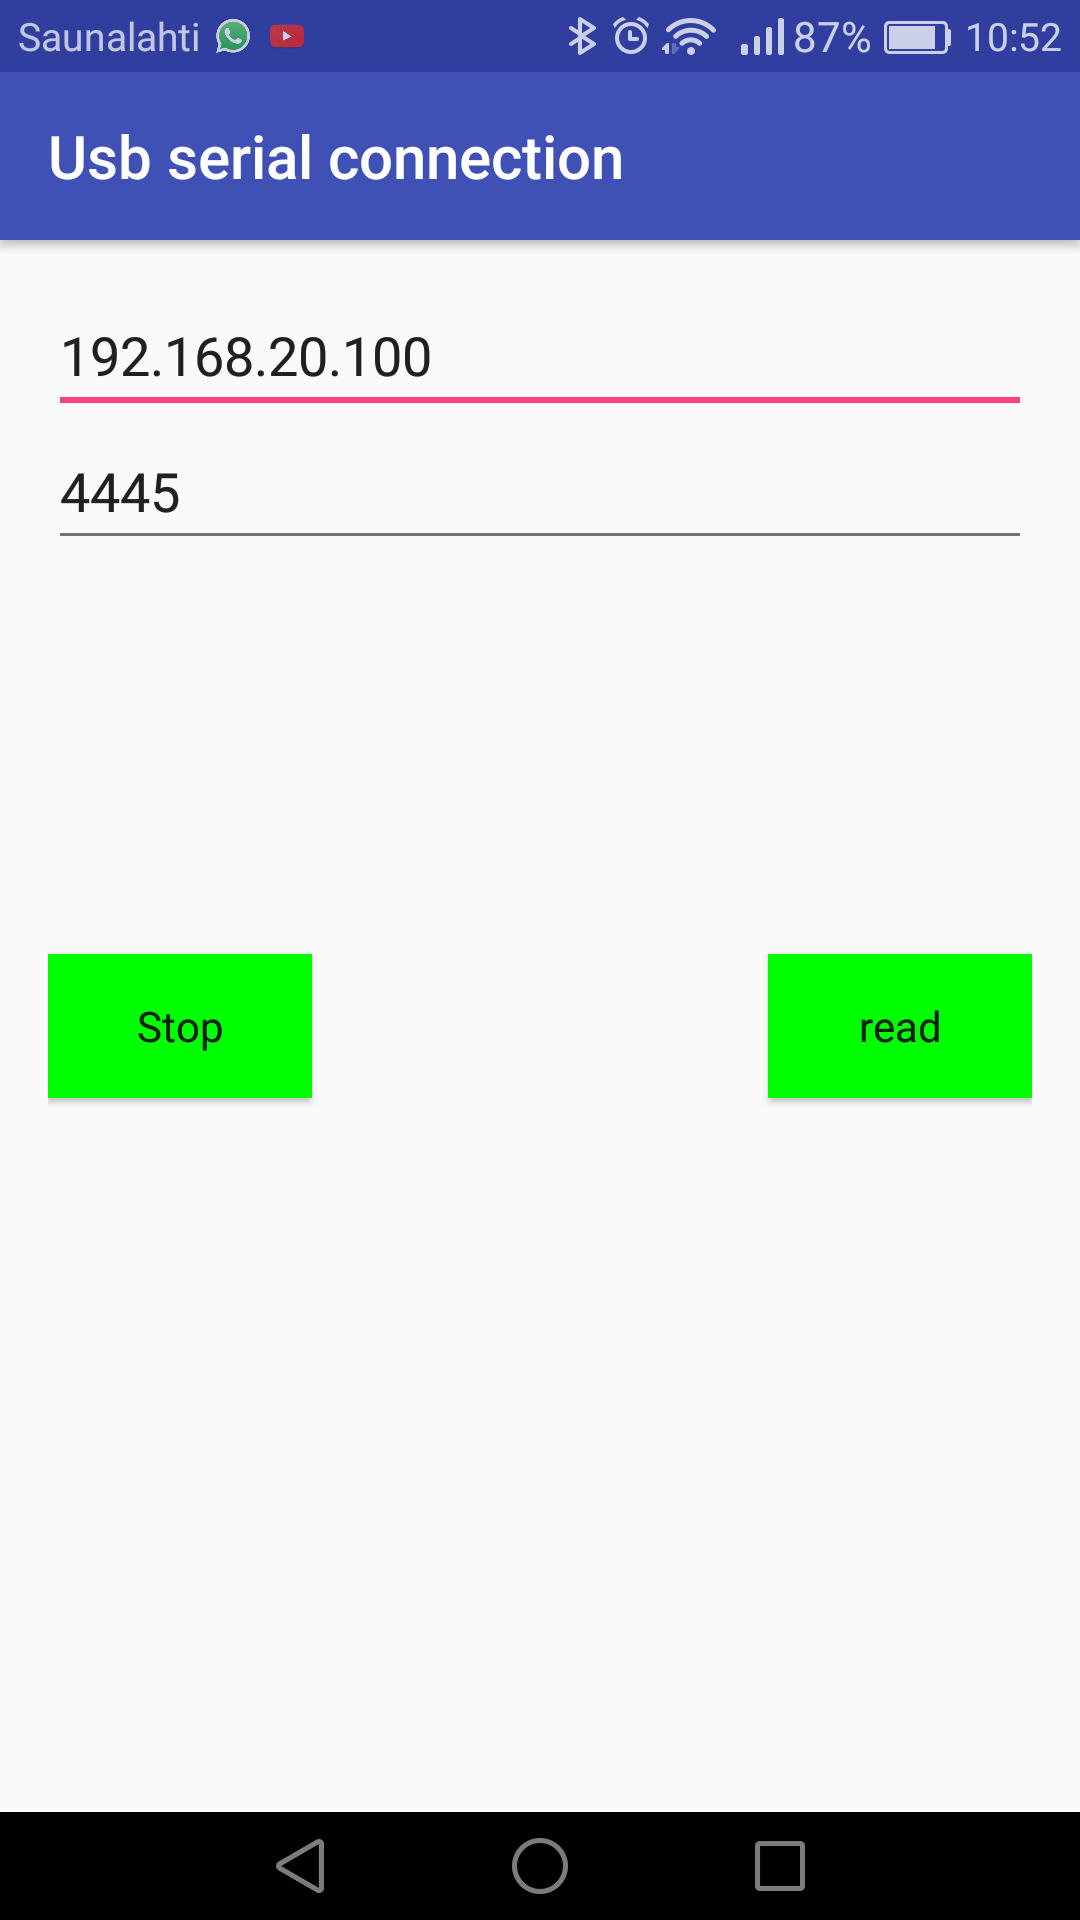
\includegraphics[width=7.1cm]{android_screenshot}
	\caption{\gls{ui} of the Android Application}
	\label{fig:android-screentshot}
\end{figure}

As network protocol \gls{http} was chosen, although it is not the best for continuously sending data. Then an \gls{php} script processed the request and store the data in a file

\begin{lstlisting}[language=PHP,basicstyle=\ttfamily,caption={PHP script on server},label=android_php_script]
<?php
$data = "";
// get data only from post request
if ($_SERVER["REQUEST_METHOD"] == "POST") {
	$data = ($_POST["data"]);
}
// write it to file
$fileName = "data.txt";
$file = fopen($fileName, "a");
if($file){
	fwrite($file, formatData($data).",");
	fclose($file);
	echo "OK";
}

function formatData($data){
	$arr = unpack('H*', $data);
	return strtoupper(implode(" ", $arr));
}
?>
\end{lstlisting}\vspace{-17pt}

Then using an Android service to keep reading in the background which is the usual approach to deal with long running operations on Android Applications.

The usb-serial-for-android library provides all the necessary to read data from the mini-usb port. The figure shows an example of implementing the callback to receive data in Java

\begin{lstlisting}[language=Java,basicstyle=\ttfamily,caption={Callback to receive data from sensor, the whole code can be accessed in \url{https://github.com/alvaro893/Android_serial_usb_communication}},label=android callback]
// the parameter data is a binary string from the sensor
@Override
public void onNewData(final byte[] data) {
	if(bufferFrames.isFull()){
			callback.getBuffer(bufferFrames);
			bufferFrames = new BufferFrames();
	}else{
			bufferFrames.addChunk(new Chunk(data));
	}
}
\end{lstlisting}\vspace{-17pt}



\subsection{Lte module}
\gls{lte} modules work as a phone: They need a \gls{sim} card to connect to network, they can be integrated in a board. Typically these modules have a number of interfaces such as \gls{usb}, rs-232, \gls{spi}, etc to connect peripherals.

In order to set a route between your device and a service on Internet or your own server, a piece of code must be provided, it depends on the module how can be done. For a project like this it is interesting that the module has its own tcp/ip stack.

The module used is configured using the Hayes command set (also called AT commands) which are used typically on modems %reference%.
This module can be programmed using \gls{javame} which is a \gls{java} edition for embedded devices \cite{javame}



\subsection{Raspberry Pi}


\chapter{Results}
\section{android smart-phone gateway solution}
This method was purely to test the sensors and to seek for a suitable network protocol rather than as a serious solution for the purposes of this thesis, nevertheless the outcomes were satisfactory and opened the door to a deeper understanding on how \gls{usb} communication can work using a High level language as \gls{java}.



\chapter{Discussion}



\chapter{Conclusions}






%----------------------------------------------------------------------------------------
%   BIBLIOGRAPHY 
%----------------------------------------------------------------------------------------

\IfLanguageName{finnish}{\bibliographystyle{vancouver_fi}}{\bibliographystyle{vancouver}}
%line space
%\singlespacing %removed otherwise the appendix are also single space
\begin{flushleft}
\begin{singlespacing}
\bibliography{biblio}
\end{singlespacing}
\end{flushleft}

%for conting the pages
\label{LastPage}~


%----------------------------------------------------------------------------------------
%   APPENDICES 
%----------------------------------------------------------------------------------------
%avoid that the last page of bib get appendix header
\clearpage
%start appendix
\appendix
%no page number for appendix in table of content
\addtocontents{toc}{\cftpagenumbersoff{chapter}}
%appendix sections and subsections not in table of content
\settocdepth{chapter}
%add "Appendices" in the table of content
\addappheadtotoc
%force smaller vertical spacing in table of content
%!!! There can be some fun depending if the appendices have (sub)sections or not :D
% You will have to play with these numbers and eventually copy the \pretocmd line on before some \chapter and force another number.
\addtocontents{toc}{\vspace{11pt}}
\pretocmd{\chapter}{\addtocontents{toc}{\protect\vspace{-24pt}}}{}{}
%have Appendix 1 (instead of Appendix A)
\renewcommand{\thechapter}{\arabic{chapter}} 

\newcommand\liite[1]{
%each appendix restart page num to one
\setcounter{page}{1}
%special counter for appendix TODO: this is a ugly quick hack :( Should find a better way to count the page per appendix.
\newtotcounter{appx#1}
%overwrite the header
\makeevenhead{plain}{}{}{\appname \thechapter \\ \thepage\,(\stepcounter{appx#1}\total{appx#1})}
\makeoddhead{plain}{}{}{\appname \thechapter \\ \thepage\,(\stepcounter{appx#1}\total{appx#1})}}

\liite{1}
\chapter{Appendix}\label{appx:first}

% Note that every appendix will be a chapter.

% Sorry for the ugly hack on how to count the total pages per appendix.


% Of course with section and subsection.

\section{Appendix Section}

% And you can cite \cite{tobias:book} stuff, it will go into the main bibliography.

\subsection{With a Subsection}

\clearpage % avoid that the last page of previous appendix get this header
\liite{2}



\chapter{Appendix 2}\label{appx:second}
\addtocontents{toc}{\vspace{11pt}}

content here 

\clearpage
\liite{3}
\end{document}
